\section{Approach}
\subsection{Overview}

To properly evaluate DFR tools, we must see how they perform in various file recovery scenarios.
We do this by running the tools on various \emph{disk images}, each containing a file system with some deleted files.
The recovered files output by a DFR tool are examined to see how well the tool meets the NIST guidelines for deleted file recovery.
By using test images designed to each emphasize specific recovery tasks, we can get a sense of a tools' strengths and weaknesses, and what tasks are especially difficult for certain types of tools.
With this in mind, we designed several disk images to test metadata-based DFR tools.
NIST CFTT has already designed a set of images for testing file carving tools, so we use those rather than creating our own.
A high-level illustration of our methodology can be seen in Figure~\ref{fig:overview}.


\begin{figure}[h]
    \centering
    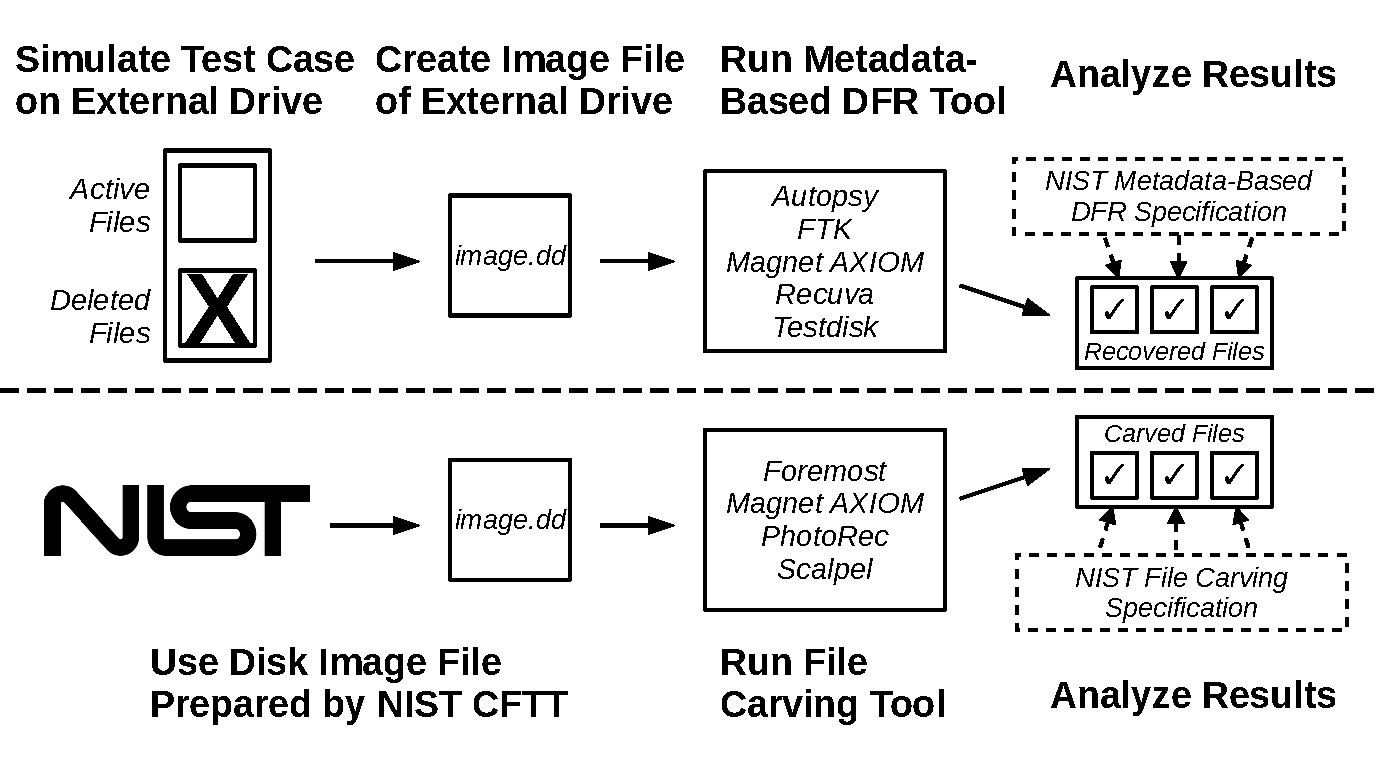
\includegraphics[width=\linewidth]{fig/overview.pdf}
    \caption{
        A read-only \emph{disk image}, a file which contains the raw data of a file system, is obtained for each test case.
        For metatada-based test cases, we create a file system on an external drive and delete files from it, then save it as a disk image.
        For file carving test cases, we use a set of disk images prepared by NIST CFTT.
        In either case disk image is input to a DFR tool, whose output is checked for compliance with the NIST guidelines for metadata-based DFR or file carving, depending on the tool.
    }
    \label{fig:overview}
\end{figure}

\subsection{Metadata-Based Tools}
\subsubsection{Designing Recovery Scenarios}

We begin by designing a set of test cases to simulate common challenges of metadata-based deleted file recovery.
In order to get the most information possible about each tools' capabilities, we design our test cases to be atomic.
We first isolate the most basic challenges of file recovery, and create test cases for them.
Then, we create test cases which combine those basic challenges.
Our intention with this atomic approach is to create test cases that are generalizeable to the majority of recovery scenarios, even the many which we do not explicitly cover.

In addition to this philosophy, we must remain within the scope of the NIST guidelines.
NIST requires test images to be ``created and deleted in a process similar to how an end-user would create and delete files.''~\cite{meta:dfr:standards}
We take this to mean that any interaction with the file system must be through a standard operating systems'  read and write operations.
We are not allowed to edit the file system directly, as ``files and file system metadata that is specifically corrupted, modified, or otherwise manipulated to appear deleted''~\cite{meta:dfr:standards} are explicitly out of scope.

Within these constraints, we can induce two phenomena which make file recovery more challenging: fragmentation and overwriting.
Following the afforementioned goal of making our tests atomic, all our test cases (besides the first trivial case) use fragmented and/or overwritten files as building blocks.
As such, our test cases fall into five general categories:
{\bf(a)} no fragmentation or overwriting, 
{\bf (b)} only fragmentation,
{\bf (c)} only overwriting,
{\bf (d)} both fragmentation and overwriting,
and {\bf (e)} fragmentation ``out of order.''


Following is a description of each test case. A selection of test cases are illustrated, with each column portraying the state of the file system at a point in time. Each file is given a unique letter and shading, and the start and end of a fragmented file are denoted when relevant.

\paragraph{Basic Deleted File}
\begin{arabiclist}
    \item Deleted file is contiguous and the only file on the disk
\end{arabiclist}
\paragraph{Deleted File is Fragmented}
\begin{arabiclist}[2]
\setcounter{enumi}{1}
    \begin{figure}
        \centering
        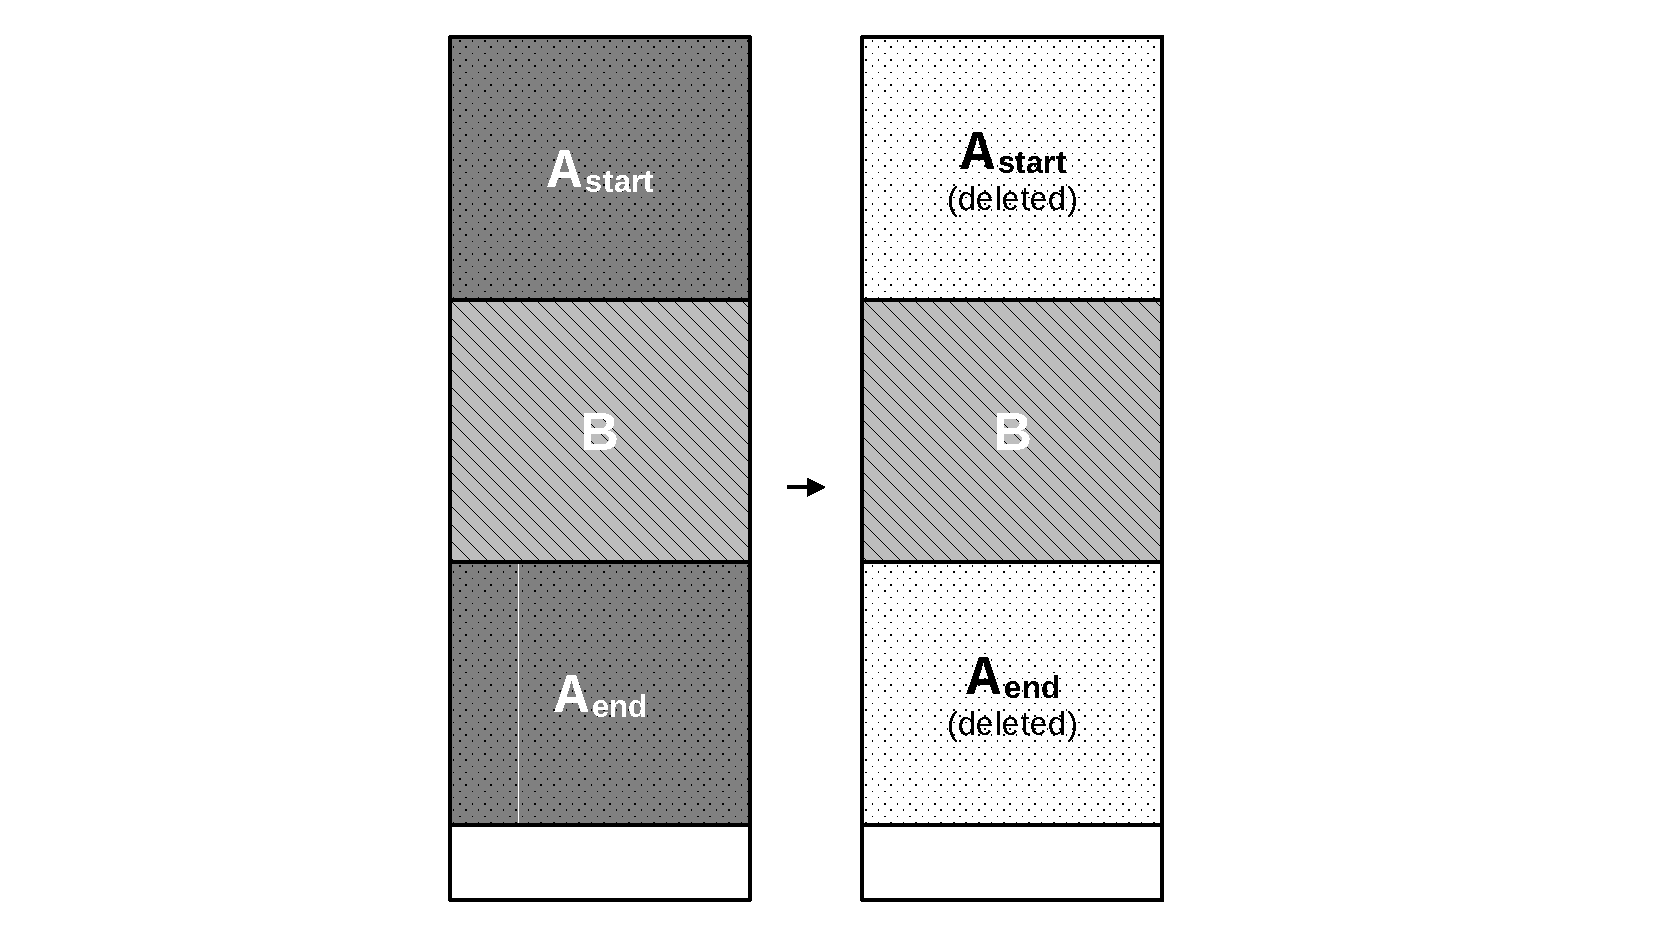
\includegraphics[width=\linewidth]{fig/case2.pdf}
        \caption{Disk 2. File A is fragmented, and has been deleted.}
        \label{fig:case2}
    \end{figure}
    \item Deleted file is fragmented around an active file (as illustrated in Figure~\ref{fig:case2})
    \item Deleted file is fragmented around another deleted file
\end{arabiclist}
\paragraph{Deleted File is Overwritten}
\begin{arabiclist}
\setcounter{enumi}{3}
    \begin{figure}
        \centering
        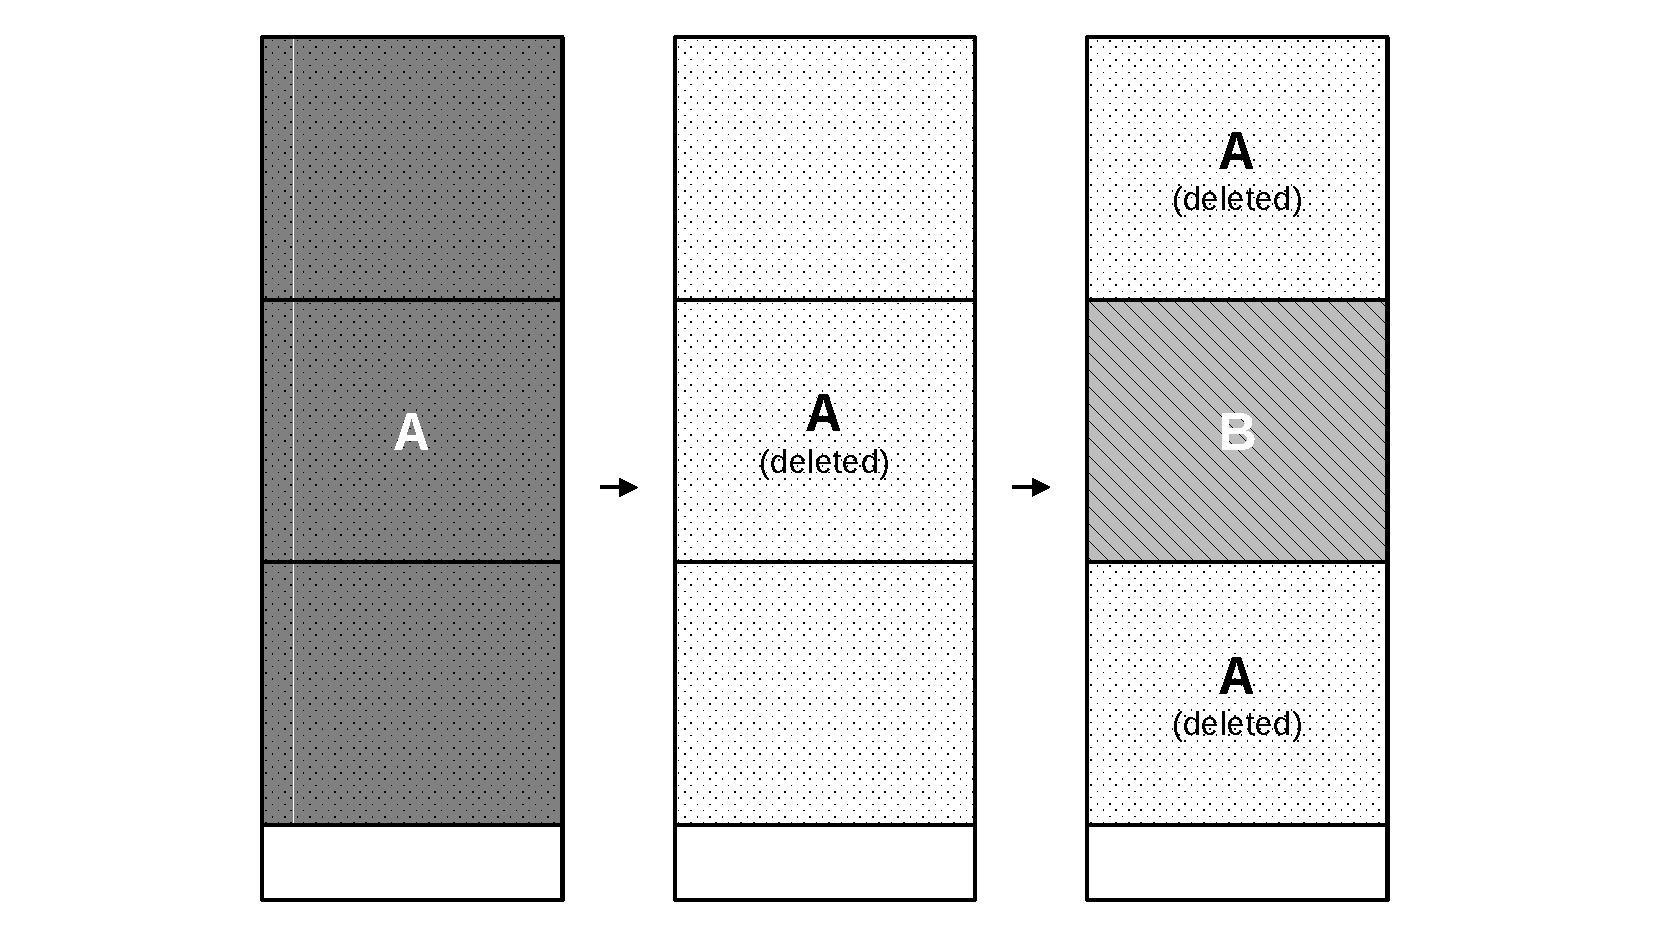
\includegraphics[width=\linewidth]{fig/case5.pdf}
        \caption{Disk 5. File A has been deleted and partially overwritten by file B.}
        \label{fig:case5}
    \end{figure}
    \begin{figure}[h]
        \centering
        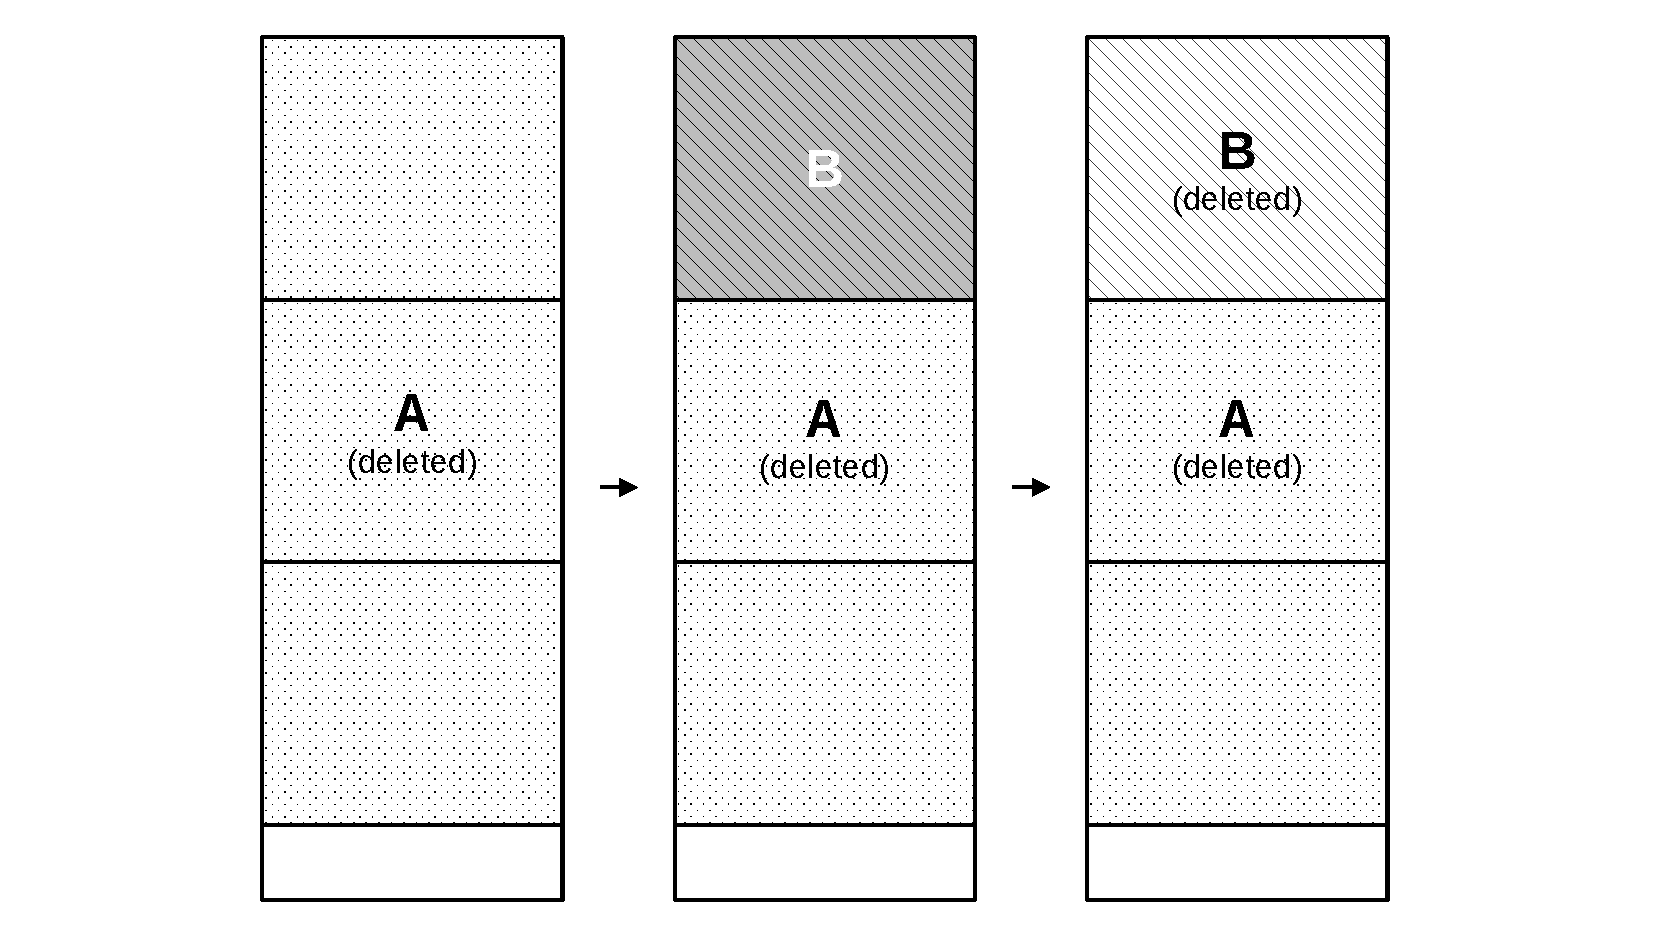
\includegraphics[width=\linewidth]{fig/case8.pdf}
        \caption{Disk 8. File A has been deleted and partially overwritten by file B, which has since been deleted}
        \label{fig:case8}
    \end{figure}
    \item Deleted file is overwritten at the front by an active file
    \item Deleted file is overwritten in the middle by an active file (as illustrated in Figure~\ref{fig:case5})
    \item Deleted file is overwritten by an active file that does not end on a sector boundary (size is not a multiple of 512 bytes)
    \item Deleted file is completely overwritten by an active file
    \item Deleted file is overwritten at the front by another deleted file (as illustrated in Figure~\ref{fig:case8})
    \item Deleted file is overwritten in the middle by another deleted file
    \item Deleted file is overwritten by another deleted file that does not end on a sector boundary (size is not a multiple of 512 bytes)
    \item Deleted file completely overwritten by another deleted file
\end{arabiclist}
\paragraph{Deleted File is Fragmented and Overwritten}
 \begin{arabiclist}
 \setcounter{enumi}{11}
     \begin{figure}[h]
        \centering
        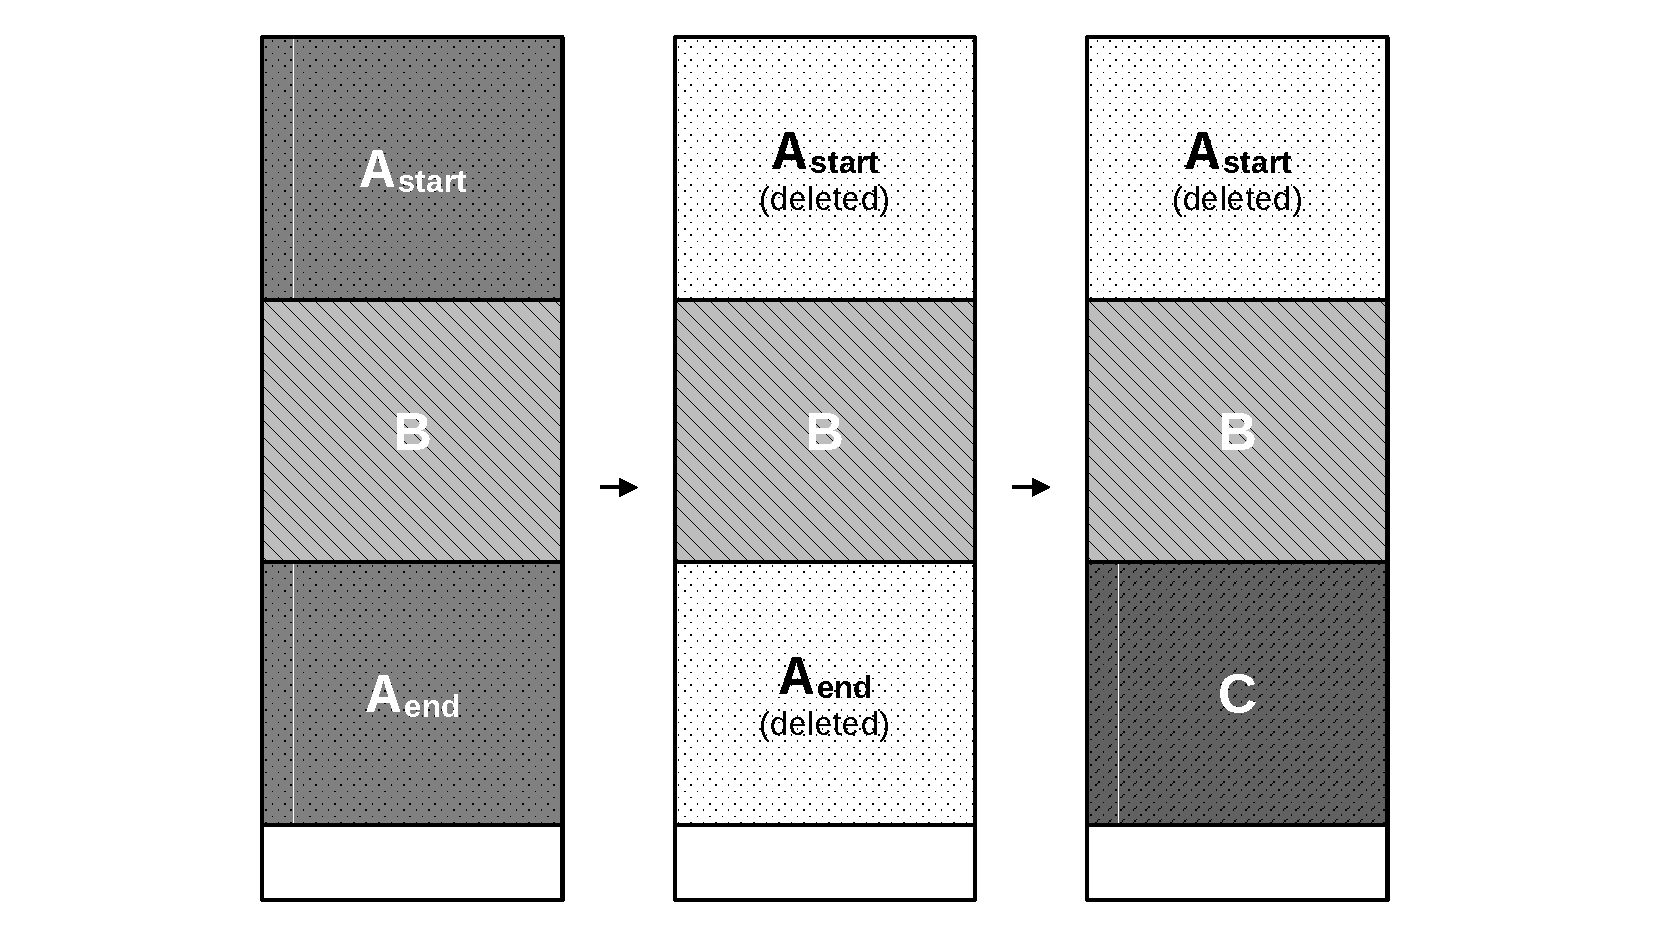
\includegraphics[width=\linewidth]{fig/case12.pdf}
        \caption{Disk 12. File A is fragmented and has been deleted. The second fragment has then been overwritten by file C}
        \label{fig:case12}
    \end{figure}
    \item Deleted file is fragmented around an active file, and the second fragment is overwritten by another active file (as illustrated in Figure~\ref{fig:case12})
    \item Deleted file is fragmented around an active file, and the second fragment is overwritten by another deleted file
 \end{arabiclist}

\paragraph{Deleted File is Fragmented Out-of-Order}
\begin{arabiclist}
\setcounter{enumi}{13}
    \begin{figure}[h]
        \centering
        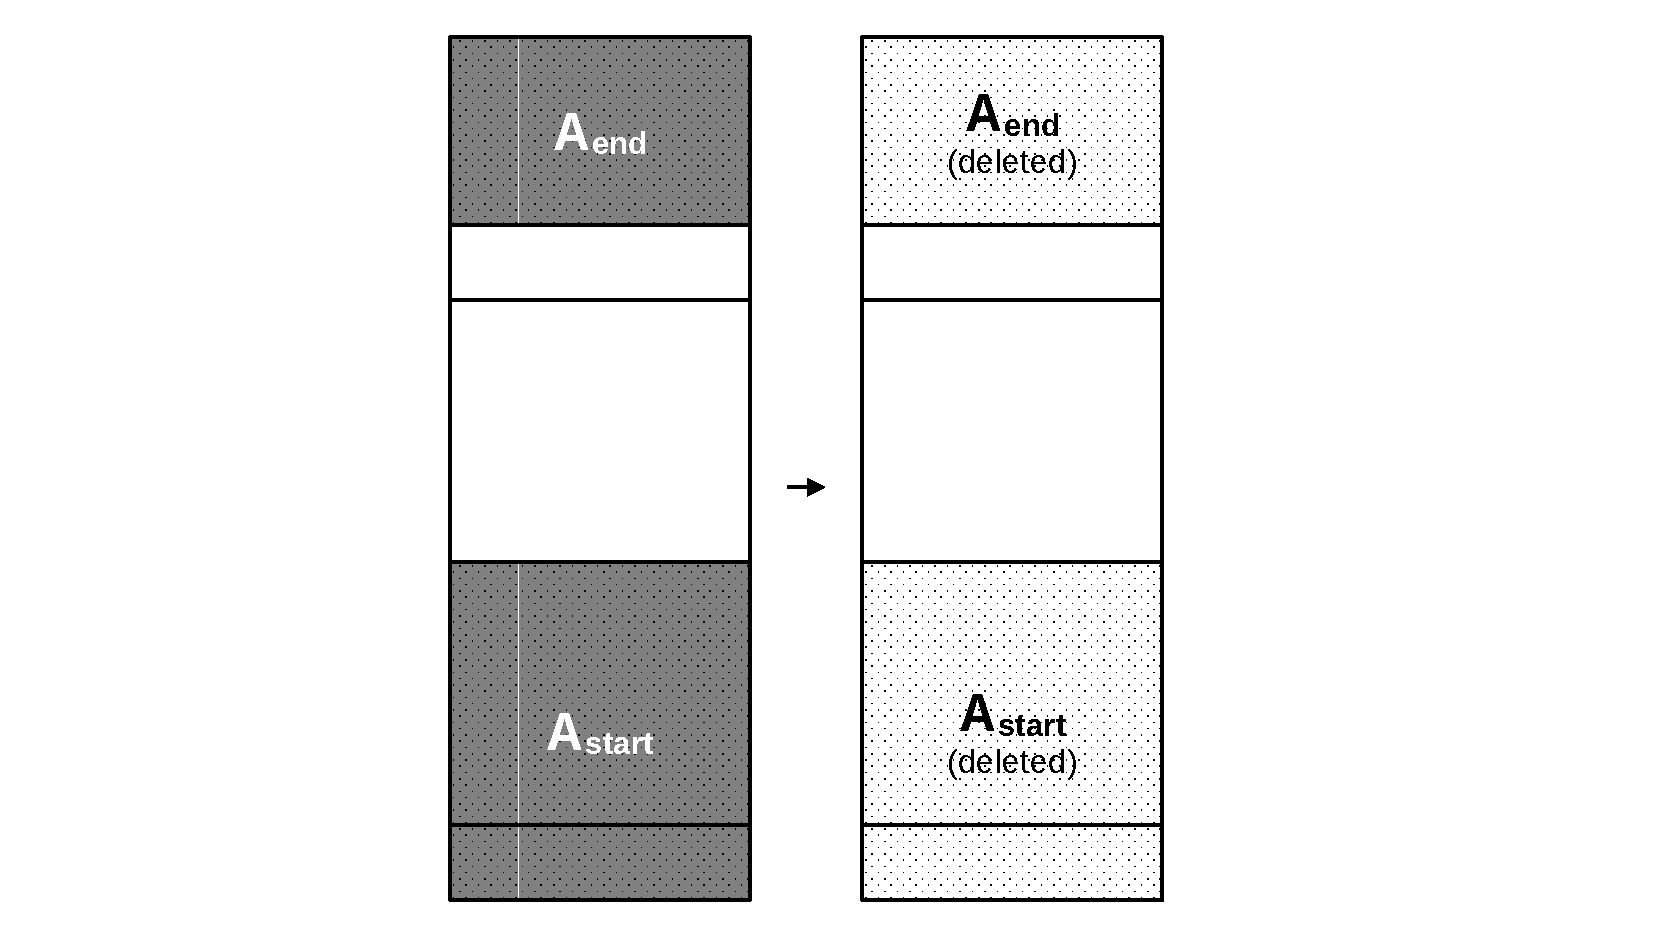
\includegraphics[width=\linewidth]{fig/case14.pdf}
        \caption{Disk 14. File A is fragmented out-of-order, and has been deleted}
        \label{fig:case14}
    \end{figure}
    \item Deleted file fragmented out-of-order (as illustrated in Figure~\ref{fig:case14})
    \item Deleted file fragmented out-of-order with an active file in between the fragments
    \item eleted file fragmented out-of-order with a deleted file in between the fragments
\end{arabiclist}



Fragmentation is trivial in NTFS because information about the runs of a file persist after deletion.
Since this renders Cases 2, 3, 14, 15, and 16 functionally identical, we only test Cases 2 and 3 for NTFS.
Cases 5 and 9 cannot be created through regular file operations in NTFS, due to NTFS's file allocation behavior.
Thus, we also exclude Cases 5 and 9 for NTFS.
We do not exclude any test cases when using FAT.


\subsubsection{Creating Test Images}

\begin{paraphrase}
 All test file systems were created in partitions on a 32 GB flash drive. For each test case, the first step is to entirely write over the partition with zeros. This ensures all cases start from identical, reproduceable conditions. A new file system is written to the partition, then files are written to the file system and deleted. The files used are simple text files containing one letter repeated (e.g., ``aa1M'' is 1 MiB of the letter `a').
 \end{paraphrase}
 Note that text files cannot be recovered with file carving, so this will force tools which combine both DFR methods to rely solely on metadata-based recovery.
 \begin{paraphrase}
 Files are written to the test file system by simply copying them from another drive. In some cases we also append data to a file in the test file system to create fragmentation. Once the test file system matches the intended scenario, a read-only image of the partition is created. All tests are performed on these images rather than the original drive. Note that when creating FAT test cases we use Ubuntu 18.04 and for NTFS test cases we use Windows 10.
\end{paraphrase}

\subsubsection{Challenges}

\begin{paraphrase}
 % Caching problem
It is important to consider when creating test images that the low-level behavior of file operations is not always obvious. For example, when writing a file, there is no guarantee the file's data will be immediately written to the disk. The operating system may cache the operation and wait until the optimal time to perform the write, in order to maximize system performance. We observed this early on, as writing a file and subsequently deleting it would always result in the file's metadata being written, but often left no evidence of the file's data having ever existed. This behavior is obviously undesirable because it leaves nothing meaningful to be recovered. We resolved this by using the \emph{sync} system call, which causes any such cached data to be immediately written to the disk, in between file writes and deletions. Unmounting the file system after writes has a similar effect.

% Learning and using the allocation algorithms
Another type of low-level behavior relevant to the image creation process is the allocation algorithm. The operating system must have some kind of algorithm to decide where in the data area new files should be written. Common allocation algorithms include ``first available,'' ``next available,'' and ``best fit.''
Learning and understanding whatever algorithm the OS uses is very helpful for forcing a specific arrangement of files. We observed that when writing to a FAT file system, Linux uses a ``next available'' algorithm. After the file system is mounted, the first write will start at the first free space in the data area. The next file will be written starting from the first free space after the previous file.
Meanwhile, when writing to an NTFS file system, Windows 10 appears to use a ``best fit'' algorithm. In this case, Windows tries to find the smallest space in which the file can fit without being fragmented, and write it there.
\end{paraphrase}

\subsubsection{Recovering Files}
\begin{paraphrase}
 We selected five popular DFR tools for testing: Autopsy~\cite{autopsy}, Recuva~\cite{recuva}, FTK Imager~\cite{ftk}, TestDisk~\cite{testdisk}, and Magnet AXIOM~\cite{axiom}. 
Note that Autopsy uses a set of DF tools known as The Sleuth Kit (TSK) for metadata-based recovery, so TSK is also implicitly covered by this study. 
These tools were chosen based on popularity and availability.
We also made sure to choose a combination of free and proprietary tools, in order to address one of the research questions.

The settings we used when testing each tool are as follows:
For Autopsy, we performed a standard recovery with all ingest modules disabled.
For Recuva we performed a standard recovery using the free version with default settings.
For FTK Imager, we performed a standard recovery using the free version with default settings.
For TestDisk we used the ``file undelete'' feature under ``Advanced Filesystem Utils.''
For Magnet AXIOM we performed a ``full scan'' in AXIOM Process and exported all files accessible in ``Filesystem View'' in AXIOM Examine.
\end{paraphrase}

\subsubsection{Results}
\begin{paraphrase}

\begin{figure}
    \centering

    \begin{subfigure}[t]{0.17\linewidth}
        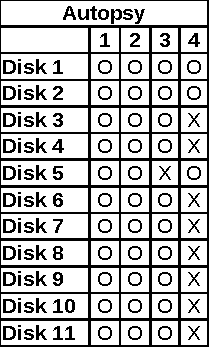
\includegraphics[width=\linewidth]{fig/autopsy_results_fat.pdf}
        \subcaption{Autopsy}
    \end{subfigure}~~
    \begin{subfigure}[t]{0.17\linewidth}
        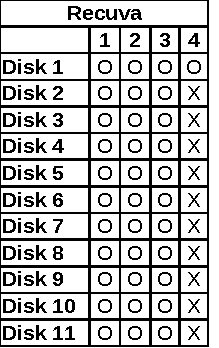
\includegraphics[width=\linewidth]{fig/recuva_results_fat.pdf}
        \subcaption{Recuva}
    \end{subfigure}~~
    \begin{subfigure}[t]{0.17\linewidth}
        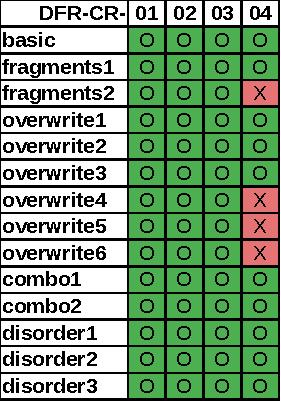
\includegraphics[width=\linewidth]{fig/ftk_results_fat.pdf}
        \subcaption{FTK}
    \end{subfigure}~~
    \begin{subfigure}[t]{0.17\linewidth}
        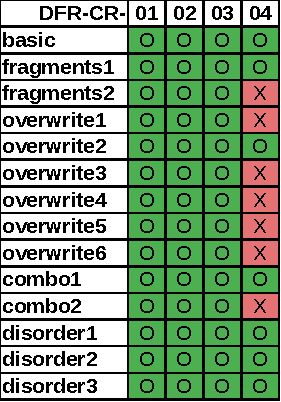
\includegraphics[width=\linewidth]{fig/testdisk_results_fat.pdf}
        \subcaption{TestDisk}
    \end{subfigure}~~
    \begin{subfigure}[t]{0.17\linewidth}
        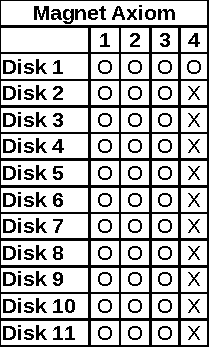
\includegraphics[width=\linewidth]{fig/axiom_results_fat.pdf}
        \subcaption{Magnet AXIOM}
    \end{subfigure}~~
        
    \caption{Test results on metadata-based DFR tools using FAT-formatted test images. Each row corresponds to a test image and each collumn corresponds to a core feature. An 'O' indicates success and an 'X' indicates failure.}
    \label{fig:results_fat}
\end{figure}

\begin{figure}
    \centering

    \begin{subfigure}[t]{0.17\linewidth}
        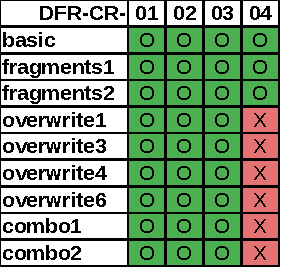
\includegraphics[width=\linewidth]{fig/autopsy_results_ntfs.pdf}
        \subcaption{Autopsy}
    \end{subfigure}~~
    \begin{subfigure}[t]{0.17\linewidth}
        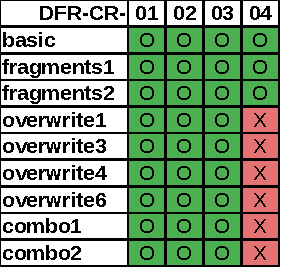
\includegraphics[width=\linewidth]{fig/recuva_results_ntfs.pdf}
        \subcaption{Recuva}
    \end{subfigure}~~
    \begin{subfigure}[t]{0.17\linewidth}
        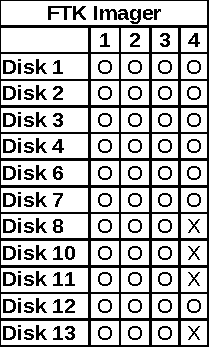
\includegraphics[width=\linewidth]{fig/ftk_results_ntfs.pdf}
        \subcaption{FTK}
    \end{subfigure}~~
    \begin{subfigure}[t]{0.17\linewidth}
        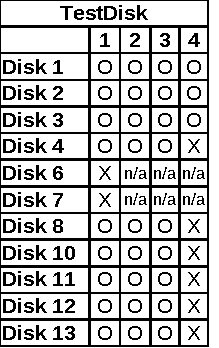
\includegraphics[width=\linewidth]{fig/testdisk_results_ntfs.pdf}
        \subcaption{TestDisk}
    \end{subfigure}~~
    \begin{subfigure}[t]{0.17\linewidth}
        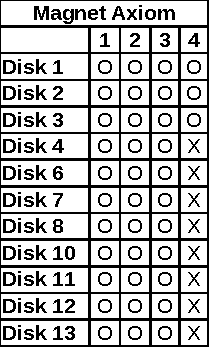
\includegraphics[width=\linewidth]{fig/axiom_results_ntfs.pdf}
        \subcaption{Magnet AXIOM}
    \end{subfigure}~~
        
    \caption{Test results on metadata-based DFR tools using NTFS-formatted test images. Each row corresponds to a test image and each collumn corresponds to a core feature. An 'O' indicates success and an 'X' indicates failure.}
    \label{fig:results_ntfs}
\end{figure}

 After testing each tool, we analyzed the recovered object(s) from each test case. 
If the recovered file is identical to the original, obviously all expectations have been met. 
While this is ideal, it is often impossible to perfectly recover a file (such as when it is overwritten) so the standards do not require it. 

In our results, the file is only ever recovered perfectly in FAT cases 1 and 2, and NTFS cases 1-3. 
For all other cases, the tool is judged on each core feature individually. 
These judgments are summarized in Figure~\ref{fig:results_fat} for FAT test cases and Figure~\ref{fig:results_ntfs} for NTFS test cases.

For cases in which a tool does not fulfill core feature 1, in other words, it cannot find a deleted file, we make no judgment about the remaining core features.

\paragraph{Recovering Fragmented Files}
In cases of fragmentation in FAT file systems, we found each tool generally approaches recovery in one of two ways. 
Recuva and Magnet AXIOM start from the beginning of the file and recover the full length of the file even if an active file exists in that space. 
Autopsy, FTK, and TestDisk will start from the beginning of the file and recover the full length, but skip over any active files they encounter.
Autopsy, FTK, and TestDisk recover all of file A, while Recuva and Magnet AXIOM's recovered images erroneously contain data from file B, causing them to fail core feature 4. 
When the space in between fragments is unallocated, all tools recover the file as though it was contiguous, pulling some erroneous data and failing core feature 4. 
When the fragmentation occurs at the end of the file system, Recuva, FTK, and TestDisk recover only the first fragment, while Autopsy returns a short file of null data, and Magnet AXIOM reports an error and returns an empty file.
Cases with fragmentation are trivial for NTFS file systems as more information is available from the metadata. 
Unsurprisingly, no tools had problems with fragmentation cases for NTFS.

\paragraph{Recovering Overwritten Files}
In cases where a file has been overwritten by an active file, we found most tools recover the deleted file as though it is not overwritten, failing core feature 4. 
A few exceptions are FTK Imager, which recovers the file up to the point where it has been overwritten, and Autopsy, which generally recovers only the first cluster of an overwritten file in FAT, and behaves like the other tools for NTFS. 
TestDisk also exhibits the same behavior as FTK for FAT case 4ii only. 
Strangely, Magnet AXIOM's recovered objects for FAT cases 4i and 4ii include the overwritten sections, but nothing after them.
Other Magnet AXIOM results were similar to the other tools.
When the overwriting file has also been deleted, all tools recover the first file as though it is not overwritten.

\paragraph{Abnormal Results}
A few results stand out as unusual.
These are cases for which it is difficult to infer from the recovered object what approach a tool is using.

For FAT cases 4ii, 6, 8, 9, and 10, Autopsy returns a 1.5 KiB file of null data.
1.5 KiB is equivalent to 3 sectors, while a FAT cluster in our cases is defined as 4 sectors (2 KiB).

TestDisk fails to identify a file for NTFS cases 4iii and 4iv only. 
These are the only test cases in which a tool does not fulfill core feature 1.

For FAT cases 4i and 4ii, Magnet AXIOM does not recover the entire length of the deleted file, but it also does not exclude the overwritten sections. 
In both cases, it recovers up to the end of the overwritten sections, rather than up to the beginning like FTK does.
\end{paraphrase}




\subsection{Carving-Based Tools}

\subsubsection{CFTT Test Cases}
To evaluate the file carving tools, we used six disk images prepared by CFTT\cite{cftt_carving_images}.
Each of these images contains between 20 and 40 graphical files of the JPG, PNG, GIF, BMP, and TIF formats.
Importantly, the CFTT images do not contain valid file-systems.
This ensures that a tool which utilizes both DFR methods can be evaluated solely on its file carving ability.

Despite the differences between the methods, metadata-based DFR and file carving are complicated by the same two file-system behaviors: fragmentation and overwriting. Thus, the CFTT test cases are somewhat similar to the ones we created for metadata-based DFR; each is built around a specific variation of fragmentation or overwriting of deleted files.
Following are summaries of each CFTT test image:
\begin{itemize}
 \item \textbf{basic:} 40 contiguous files, with space in between each file
 \item \textbf{nofill:} 40 contiguous files, with no space in between each file
 \item \textbf{simple-frag:} 40 fragmented files, with space in between each fragment
 \item \textbf{braid:} 10 contiguous files and 10 fragmented files, which are fragmented around each other in an A-B-A-B pattern
 \item \textbf{disorder:} 35 fragmented files, 30 of which are fragmented out-of-order such that the fragment containing the footer comes before the fragment containing the header
 \item \textbf{partials:} 15 complete files, 5 of which are fragmented, and 25 incomplete files where at least one fragment has been overwritten or manually destroyed

\end{itemize}


\subsubsection{Recovering Files}

 We selected four popular file carving tools for testing: PhotoRec~\cite{photorec}, Foremost~\cite{foremost}, Scalpel~\cite{scalpel}, and Magnet AXIOM~\cite{axiom}.

The settings we used when testing each tool are as follows:
For PhotoRec and Foremost, we used the default settings.
For Scalpel, we manually enabled recovery of the JPG, PNG, GIF, BMP, and TIF formats, and otherwise used default settings.
For Magnet Axiom, we ran a ``full scan'' with default settings in AXIOM Process and exported all graphical files from ``Artifact View'' in AXIOM Examine.
We also exported an XML carving report from Axiom Examine as unlike the other tools it does not create one automatically.

\subsubsection{Evaluating Results}
The main challenge when testing file carving tools is verifying the results. 
For metadata-based tools this is fairly simple; the deleted files in our tests are all simple text files which can be checked at a glance.
However, text files lack a standard header and footer and thus cannot be recovered with file carving, so the test images use more complicated formats such as JPG.
As a result, it would be impractical to evaluate a tool based on the carved files alone.

Fortunately, all four of the carving tools we evaluated produce an itemized report of carving results. CFTT provides detailed information about the contents of the test images, so we can compare the tools' reports with the true arrangement of files in each image. This is particularly important for core feature 1, core feature 2, and core feature 3 since they are concerned with the specific data blocks the tool carves. PhotoRec's report gives a start and end address for each file, and multiple start and end addresses if it attempts to carve a fragmented file. The other tools' reports only list the starting address and size of each file, so we assumed they never attempt to carve more than one fragment per file.

Checking core feature 4 is slightly complicated by the fact that carving tools cannot recover the filename, but we can use the first sector listed for each file in the carving report to match them with the original files and check the file extensions.

For core feature 5, we make use of the \emph{identify} command from the ImageMagick~\cite{imagemagick} tool suite. Upon input of a graphical file, identify will output the file format and other information. Relevant to core feature 5 is that the return code will indicate whether the file is valid or corrupt. We add the \emph{-regard-warnings} flag so an error or warning while parsing the file will mean the file is considerd corrupt.

\subsubsection{Results}

\begin{figure}
    \centering

    \begin{subfigure}{\linewidth}
        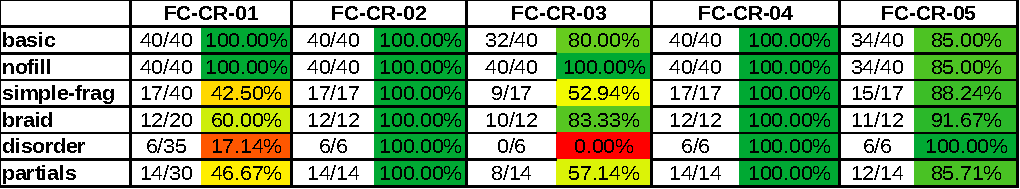
\includegraphics[width=\linewidth]{fig/photorec_results_carve.pdf}
        \subcaption{PhotoRec}
    \end{subfigure}
    \begin{subfigure}{\linewidth}
        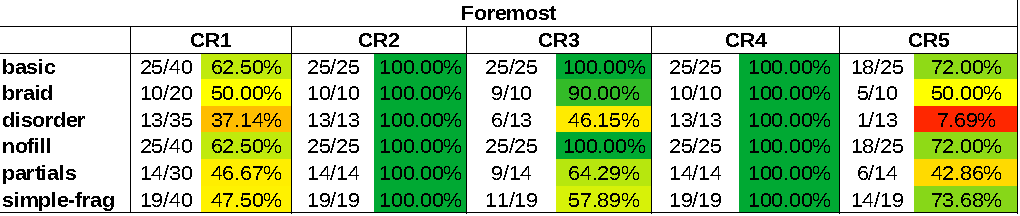
\includegraphics[width=\linewidth]{fig/foremost_results_carve.pdf}
        \subcaption{Foremost}
    \end{subfigure}
    \begin{subfigure}{\linewidth}
        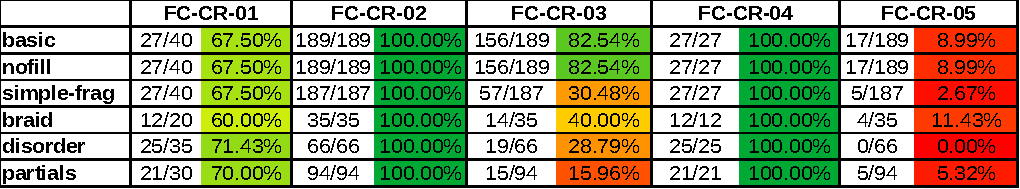
\includegraphics[width=\linewidth]{fig/scalpel_results_carve.pdf}
        \subcaption{Scalpel}
    \end{subfigure}
    \begin{subfigure}{\linewidth}
        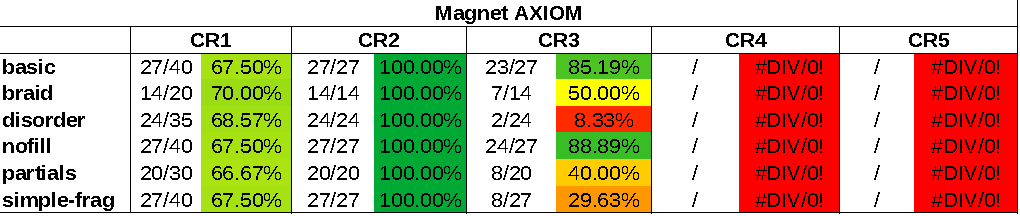
\includegraphics[width=\linewidth]{fig/axiom_results_carve.pdf}
        \subcaption{Magnet AXIOM}
    \end{subfigure}
        
    \caption{\TODO{working version of carving results}}
    \label{fig:results_carve}
\end{figure}

\TODO{TODO} 
